\documentclass[12pt,a4paper]{report}
% Language: English
\pdfminorversion=7
\usepackage[pdftex]{graphicx}

\begin{document}

\begin{titlepage}
\vspace{2cm}
\begin{center}
\Huge{Notes on Files in Folder \texttt{modules/ftm/ftmx86}}

\Huge{Description of Tests for Schedule Validation}

\Large{Martin Skorsky}

\Large{2020-06-25}
\end{center}
\vfill
\end{titlepage}

\tableofcontents

\chapter{Description of Tests for Schedule Validation}
The tests for the schedule validation check all rules from \texttt{src/validation.cpp}. For each rule we have a positive and a negative test. Each test is a dot file which is loaded into data master and the result is checked.

\begin{enumerate}
    \item Command switch is only allowed for blocks. This is not checked during validation. The post-mortem command uses this leak. Switch is used for a timming message.
    \item Use logging (FESA logging) of data master actions for checks in tests. 
    \item Re-use \texttt{dm-test.cpp} for testing safe removal of schedules or partial schedules.
    \item Use Boost Graphics code to generate graphs.
    \item Check each rule of the validation table. In addition check that each endless loop contains a block and time offsets of successive nodes are increasing.
    \item Read validation source: src/validation.cpp contains methods neighbourhoodCheck and eventSequenceCheck.
    \item Validation for run time commands and for schedules.
\end{enumerate}

\chapter{Description of Files}

\begin{enumerate}
\item dm-cmd, dm-cmd.cpp: Executable and source for data master command.
\item dm-sched, dm-sched.cpp: Executable and source for data master schedule loader.
\item full\_test - Folder with tests.
\item Makefile
\item carpedm\_doxy.conf: configuration for doxy
\item dm-test.cpp: Source for data master test program.
\item foo.cpp: C++ snippet, opens etherbone socket and device. Not clear where this is used.
\item before.dot
    \begin{figure}
        \centering 
        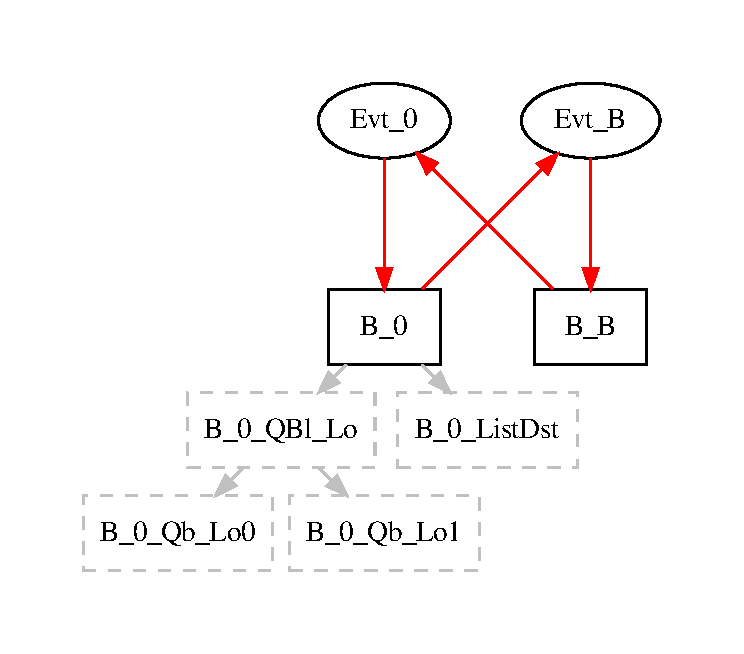
\includegraphics{TestPattern/before.pdf}
        \caption{before}
        \label{fig:before}
    \end{figure}
\item blink-test.sh: data master test script with blink.dot
\begin{verbatim}
#!/bin/bash
file=blink.dot

eb-fwload $1 u0 0 ../ftmfw/ftm.bin
sleep 1
./dm-sched $1 $file -w
sleep 1
./dm-cmd $1 $file origin -t0 Evt_POLICE0
./dm-cmd $1 $file origin -t1 Evt_FIREF0
./dm-cmd $1 $file preptime -t0 1000000000
./dm-cmd $1 $file preptime -t1 1000000000

./dm-cmd $1 $file starttime -t0 0000000
./dm-cmd $1 $file starttime -t1 0000000
./dm-cmd $1 $file start 0x3
sleep 1
./dm-cmd $1 $file heap
\end{verbatim}
\item blink.dot, see Figure~\ref{fig:blink}.
    \begin{figure}
        \centering 
        \includegraphics*[width=1.0\textwidth,keepaspectratio]{TestPattern/blink.pdf}
        \caption{blink}
        \label{fig:blink}
    \end{figure}
\item cmd\_multipat.dot, see Figure~\ref{fig:cmd_multipat}.
    \begin{figure}
        \centering 
        \includegraphics*[width=1.0\textwidth,keepaspectratio]{TestPattern/cmd_multipat.pdf}
        \caption{cmd\_multipat}
        \label{fig:cmd_multipat}
    \end{figure}
\item corrupted.dot, see Figure~\ref{fig:corrupted}.
    \begin{figure}
        \centering 
        \includegraphics*[width=1.0\textwidth,keepaspectratio]{TestPattern/corrupted.pdf}
        \caption{corrupted}
        \label{fig:corrupted}
    \end{figure}
\item tmp.dot, see Figure~\ref{fig:tmp}.
    \begin{figure}
        \centering 
        \includegraphics*[width=1.0\textwidth,keepaspectratio]{TestPattern/tmp.pdf}
        \caption{tmp}
        \label{fig:tmp}
    \end{figure}
\item duffy.dot, see Figure~\ref{fig:duffy}.
    \begin{figure}
        \centering 
        \includegraphics*[width=1.0\textwidth,keepaspectratio]{TestPattern/duffy.pdf}
        \caption{duffy}
        \label{fig:duffy}
    \end{figure}
\item duffy\_t.dot, see Figure~\ref{fig:duffy_t}.
    \begin{figure}
        \centering 
        \includegraphics*[width=1.0\textwidth,keepaspectratio]{TestPattern/duffy_t.pdf}
        \caption{duffy\_t}
        \label{fig:duffy_t}
    \end{figure}
\item inspect.dot, see Figure~\ref{fig:inspect}.
    \begin{figure}
        \centering 
        \includegraphics*[width=1.0\textwidth,keepaspectratio]{TestPattern/inspect.pdf}
        \caption{inspect}
        \label{fig:inspect}
    \end{figure}
\item multipat.dot, see Figure~\ref{fig:multipat}.
    \begin{figure}
        \centering 
        \includegraphics*[width=1.0\textwidth,keepaspectratio]{TestPattern/multipat.pdf}
        \caption{multipat}
        \label{fig:multipat}
    \end{figure}
\item multi\_schedule.dot, see Figure~\ref{fig:multi_schedule}.
    \begin{figure}
        \centering 
        \includegraphics*[width=1.0\textwidth,keepaspectratio]{TestPattern/multi_schedule.pdf}
        \caption{multi\_schedule}
        \label{fig:multi_schedule}
    \end{figure}
\item normal\_download.dot, see Figure~\ref{fig:normal_download}.
    \begin{figure}
        \centering 
        \includegraphics*[width=1.0\textwidth,keepaspectratio]{TestPattern/normal_download.pdf}
        \caption{normal\_download}
        \label{fig:normal_download}
    \end{figure}
\item pps.dot, see Figure~\ref{fig:pps}.
    \begin{figure}
        \centering 
        \includegraphics*[width=1.0\textwidth,keepaspectratio]{TestPattern/pps.pdf}
        \caption{pps}
        \label{fig:pps}
    \end{figure}
\item simple.dot, see Figure~\ref{fig:simple}.
    \begin{figure}
        \centering 
        \includegraphics*[width=1.0\textwidth,keepaspectratio]{TestPattern/simple.pdf}
        \caption{simple}
        \label{fig:simple}
    \end{figure}
\item sis\_hest.dot, see Figure~\ref{fig:sis_hest}.
    \begin{figure}
        \centering 
        \includegraphics*[width=1.0\textwidth,keepaspectratio]{TestPattern/sis_hest.pdf}
        \caption{sis\_hest}
        \label{fig:sis_hest}
    \end{figure}
\item stripped\_download.dot, see Figure~\ref{fig:stripped_download}.
    \begin{figure}
        \centering 
        \includegraphics*[width=1.0\textwidth,keepaspectratio]{TestPattern/stripped_download.pdf}
        \caption{stripped\_download}
        \label{fig:stripped_download}
    \end{figure}
\item test0\_0.dot, see Figure~\ref{fig:test0_0}.
    \begin{figure}
        \centering 
        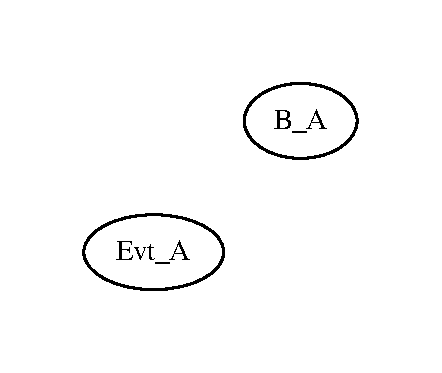
\includegraphics{TestPattern/test0_0.pdf}
        \caption{test0\_0}
        \label{fig:test0_0}
    \end{figure}
\item test0\_1.dot, see Figure~\ref{fig:test0_1}.
    \begin{figure}
        \centering 
        \includegraphics*[width=1.0\textwidth,keepaspectratio]{TestPattern/test0_1.pdf}
        \caption{test0\_1}
        \label{fig:test0_1}
    \end{figure}
\item test1\_0.dot, see Figure~\ref{fig:test1_0}.
    \begin{figure}
        \centering 
        \includegraphics*[width=1.0\textwidth,keepaspectratio]{TestPattern/test1_0.pdf}
        \caption{test1\_0}
        \label{fig:test1_0}
    \end{figure}
\item test1\_1.dot, see Figure~\ref{fig:test1_1}.
    \begin{figure}
        \centering 
        \includegraphics*[width=1.0\textwidth,keepaspectratio]{TestPattern/test1_1.pdf}
        \caption{test1\_1}
        \label{fig:test1_1}
    \end{figure}
\item test1.dot, see Figure~\ref{fig:test1}.
    \begin{figure}
        \centering 
        \includegraphics*[width=1.0\textwidth,keepaspectratio]{TestPattern/test1.pdf}
        \caption{test1}
        \label{fig:test1}
    \end{figure}
\item test2\_0.dot, see Figure~\ref{fig:test2_0}.
    \begin{figure}
        \centering 
        \includegraphics*[width=1.0\textwidth,keepaspectratio]{TestPattern/test2_0.pdf}
        \caption{test2\_0}
        \label{fig:test2_0}
    \end{figure}
\item test2\_1.dot, see Figure~\ref{fig:test2_1}.
    \begin{figure}
        \centering 
        \includegraphics*[width=1.0\textwidth,keepaspectratio]{TestPattern/test2_1.pdf}
        \caption{test2\_1}
        \label{fig:test2_1}
    \end{figure}
\item test2.dot, see Figure~\ref{fig:test2}.
    \begin{figure}
        \centering 
        \includegraphics*[width=1.0\textwidth,keepaspectratio]{TestPattern/test2.pdf}
        \caption{test2}
        \label{fig:test2}
    \end{figure}
\item test3\_0.dot, see Figure~\ref{fig:test3_0}.
    \begin{figure}
        \centering 
        \includegraphics*[width=1.0\textwidth,keepaspectratio]{TestPattern/test3_0.pdf}
        \caption{test3\_0}
        \label{fig:test3_0}
    \end{figure}
\item test3\_1.dot, see Figure~\ref{fig:test3_1}.
    \begin{figure}
        \centering 
        \includegraphics*[width=1.0\textwidth,keepaspectratio]{TestPattern/test3_1.pdf}
        \caption{test3\_1}
        \label{fig:test3_1}
    \end{figure}
\item test3\_2.dot, see Figure~\ref{fig:test3_2}.
    \begin{figure}
        \centering 
        \includegraphics*[width=1.0\textwidth,keepaspectratio]{TestPattern/test3_2.pdf}
        \caption{test3\_2}
        \label{fig:test3_2}
    \end{figure}
\item test3\_3.dot, see Figure~\ref{fig:test3_3}.
    \begin{figure}
        \centering 
        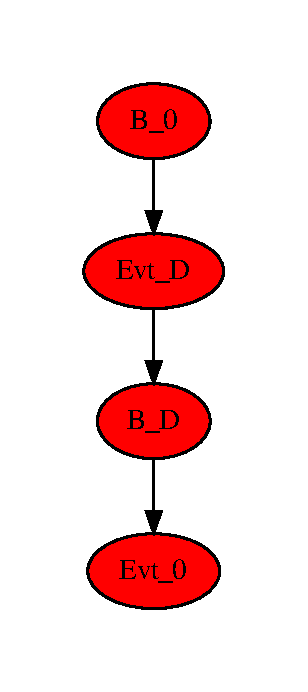
\includegraphics{TestPattern/test3_3.pdf}
        \caption{test3\_3}
        \label{fig:test3_3}
    \end{figure}
\item test3\_4.dot, see Figure~\ref{fig:test3_4}.
    \begin{figure}
        \centering 
        \includegraphics*[width=1.0\textwidth,keepaspectratio]{TestPattern/test3_4.pdf}
        \caption{test3\_4}
        \label{fig:test3_4}
    \end{figure}
\item test4\_0.dot, see Figure~\ref{fig:test4_0}.
    \begin{figure}
        \centering 
        \includegraphics*[width=1.0\textwidth,keepaspectratio]{TestPattern/test4_0.pdf}
        \caption{test4\_0}
        \label{fig:test4_0}
    \end{figure}
\item test4\_1.dot, see Figure~\ref{fig:test4_1}.
    \begin{figure}
        \centering 
        \includegraphics*[width=1.0\textwidth,keepaspectratio]{TestPattern/test4_1.pdf}
        \caption{test4\_1}
        \label{fig:test4_1}
    \end{figure}
\item test5\_0.dot, see Figure~\ref{fig:test5_0}.
    \begin{figure}
        \centering 
        \includegraphics*[width=1.0\textwidth,keepaspectratio]{TestPattern/test5_0.pdf}
        \caption{test5\_0}
        \label{fig:test5_0}
    \end{figure}
\item test5\_1.dot, see Figure~\ref{fig:test5_1}.
    \begin{figure}
        \centering 
        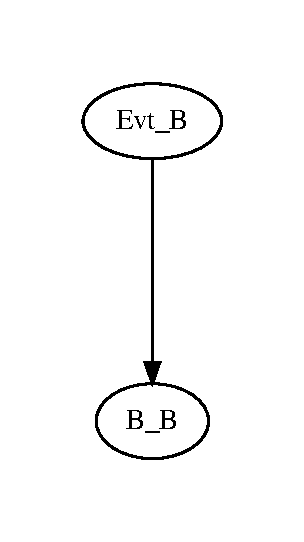
\includegraphics{TestPattern/test5_1.pdf}
        \caption{test5\_1}
        \label{fig:test5_1}
    \end{figure}
\item test\_cmd.dot, see Figure~\ref{fig:test_cmd}.
    \begin{figure}
        \centering 
        
\includegraphics{TestPattern/test_cmd.pdf}
        \caption{test\_cmd}
        \label{fig:test_cmd}
    \end{figure}
\item test.dot, see Figure~\ref{fig:test}.
    \begin{figure}
        \centering 
        \includegraphics*[width=1.0\textwidth,keepaspectratio]{TestPattern/test.pdf}
        \caption{test}
        \label{fig:test}
    \end{figure}
\item tryme.dot, see Figure~\ref{fig:tryme}.
    \begin{figure}
        \centering 
        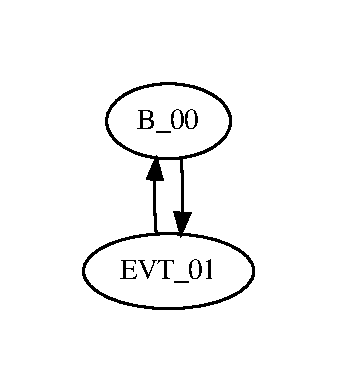
\includegraphics{TestPattern/tryme.pdf}
        \caption{tryme}
        \label{fig:tryme}
    \end{figure}
\item upload.dot, see Figure~\ref{fig:upload}.
    \begin{figure}
        \centering 
        \includegraphics*[width=1.0\textwidth,keepaspectratio]{TestPattern/upload.pdf}
        \caption{upload}
        \label{fig:upload}
    \end{figure}
\item val.dot, see Figure~\ref{fig:val}.
    \begin{figure}
        \centering 
        \includegraphics*[width=1.0\textwidth,keepaspectratio]{TestPattern/val.pdf}
        \caption{val}
        \label{fig:val}
    \end{figure}
\item dm-log-replay.py: Python script, purpose not clear.
\item dict.sh: sed script, purpose not clear.
\item neatorender.sh: renders dot files in background.
\item pro-dump.sh: dump data master in production (tsl017.acc).
\item reenact.sh: eb-write, eb-put; memory dump for all rams.
\item render.sh
\item restore\_dump.sh
\item sleep\_until\_modified.sh
\item sorted\_render.sh
\item test.sh
\item trem.sh
\item xdotneato.sh
\item download2.svg
\end{enumerate}

\end{document}
